%%%%%%%%%%%%%%%%%%%%%%%%%%%%%%%%%%%%%%%%%%%%%%%%%%%%%%%%%%%%%%%%%%%%%%%%%%%%%%%%
\chapter{Related Work}
\label{chapter:ch3-related_work}
%%%%%%%%%%%%%%%%%%%%%%%%%%%%%%%%%%%%%%%%%%%%%%%%%%%%%%%%%%%%%%%%%%%%%%%%%%%%%%%%
\localtoc


This thesis makes contributions on building compact and robust neural networks with help from Toeplitz matrix theory.
This chapter, divided in two parts, aims at presenting an overview on current works related to our contributions.
First, we present the current methods to build compact neural networks.  
Given that the scope of current techniques is large, we choose to focus mainly on works which uses tools from linear algebra and more particularly structured matrices.

Our second contribution focus on build robust neural networks by regularizing the Lipschitz constant of neural networks.
The second part of this chapter present current methods for regularizing this constant that aim to improving the robust of neural networks.
We omit methods that are orthogonal to our approach for clarity and conciseness.


%%%%%%%%%%%%%%%%%%%%%%%%%%%%%%%%%%%%%%%%%%%%%%%%%%%%%%%%%%%%%%%%%%%%%%%%%%%%%%%%
\section{Related Work on Compact Neural Networks}
\label{section:ch3-related_work_on_compact_neural_networks}
%%%%%%%%%%%%%%%%%%%%%%%%%%%%%%%%%%%%%%%%%%%%%%%%%%%%%%%%%%%%%%%%%%%%%%%%%%%%%%%%

% In this chapter, we review the literature on techniques for building compact neural networks.
% First of all, we present, in detail, related work which uses tools from linear algebra and structured matrices. 
% Finally, we present in a more concise way concurrent techniques like using specific memory representation or using neural architecture search.
% These techniques are mostly orthogonal to our contributions.


% We have seen in the Introduction (\Cref{chapter:ch2-introduction}) and Background (\Cref{chapter:ch2-background}) that neural networks tend to be over-parametrized which lead to difficult and expensive training and overfitting.


% In this section, we review the literature for building compact neural networks.
% As seen in the Introduction (\Cref{chapter:ch1-introduction}) and Background (\Cref{chapter:ch2-background}), scaling up networks can lead to an increase in accuracy.
% Researchers have demonstrated that increasing the width of shallow neural networks increased their performance~\cite{howard2017mobilenets,sandler2018mobilenetv2,tan2019mnasnet,zagoruyko2016wide} due to their capacity to capture more fine-grained features.
% Increasing depth is a common and effective way to scale neural networks and many deep architectures have been proposed~\cite{he2016deep, huang2016deep, szegedy2016rethinking,szegedy2017inception,xiao2018dynamical}. 
% The intuition is that deep neural network can capture richer and more complex features.


% Increasing the width of shallow neural networks can increase their performance~\cite{howard2017mobilenets,sandler2018mobilenetv2,tan2019mnasnet,zagoruyko2016wide} due to their capacity to capture more fine-grained features.
% As well, increasing depth is a common and effective approach to capture richer and more complex features and increase performance, many deep architectures have been proposed~\cite{he2016deep,huang2016deep, szegedy2016rethinking,szegedy2017inception,xiao2018dynamical}.
% However, large neural networks lead to difficult and expensive training and overfitting and after observing that a lot of parameters in large neural networks were redundant~\cite{dai2018compressing,frankle2018lottery}, an important question arises: \emph{do neural networks needs to be over-parameterized? And if not, how to build accurate and compact neural networks?} 

%%%%%%%%%%%%%%%%%%%%%%%%%%%%%%%%%%%%%%%%%%%%%%%%%%%%%%%%%%%%%%%%%%%%%%%%%%%%%%%%
\subsection{General Techniques to Build Compact Neural Networks}
%%%%%%%%%%%%%%%%%%%%%%%%%%%%%%%%%%%%%%%%%%%%%%%%%%%%%%%%%%%%%%%%%%%%%%%%%%%%%%%%

As seen in the Introduction (\Cref{chapter:ch1-introduction}), scaling up networks can lead to better accuracy~\cite{tan2019efficientnet,brown2020language}.
However, large neural networks lead to difficult and expensive training and after observing that a lot of parameters in large neural networks were redundant~\cite{dai2018compressing,frankle2018lottery}, an important question arises: \emph{do neural networks need to be over-parameterized? And if not, how to build accurate and compact neural networks?} 

Numerous other directions have been investigated to build compact and cost-effective neural networks without impacting the accuracy.
For example \citet{gupta2015deep,micikevicius2018mixed} have proposed to represent weights with limited numerical precision to reduce training time and memory requirements.
They used half-precision floating-point format instead of single-precision floating-point format which uses 32 bits of computer memory.
In the same direction, \citet{courbariaux2015binaryconnect} have proposed a method to train neural networks with binary weights without an important loss in the accuracy.

An important idea in model compression, proposed by~\citet{bucilua2006model}, is based on the observation that the model used for training is not required to be the same as the one used for inference.
Indeed, compressed models after training can be deployed on smartphones or IoT devices.
Based on this idea, multiple post-processing techniques have been developed: a quantization procedure which consists in converting the weights into a binary or integer formats \emph{after} the training phase~\cite{mellempudi2017ternary,rastegariECCV16}, pruning techniques~\cite{dai2018compressing,han2015deep,lin2017runtime} or sparsity regularizers~\cite{collins2014memory,dai2018compressing,liu2015sparse} which consists in removing redundant weights after training and taking advantage of the sparse structure of the weight matrices.

Sparse neural networks have also been extensively studied since the seminal work of \citet{frankle2018lottery} in which they propose the \emph{Lottery Ticket Hypothesis}. 
This hypothesis states that there exists a sparse subnetwork of a dense neural network that when trained in isolation can match the test accuracy of the original dense network after training for at most the same number of iterations. 
This hypothesis led to a series of works on sparse neural networks \cite{zhou2019deconstructing,malach2019proving,evci2020rigging}.

Moreover, \citet{ba2014deep} have empirically demonstrated that shallow neural networks can learn the complex functions previously learned by other deep neural networks.
This result led \citet{hinton2015distilling} to propose a technique called \emph{model distillation} which consists in training a large complex model using all the available data and resources to be as accurate as possible, then a smaller and more compact model is trained to approximate the first model.
Although interesting for deployment purposes, this approach still requires to train one large network and one shallow, which entails a significant training cost.

\begin{figure}[t]
  \centering
  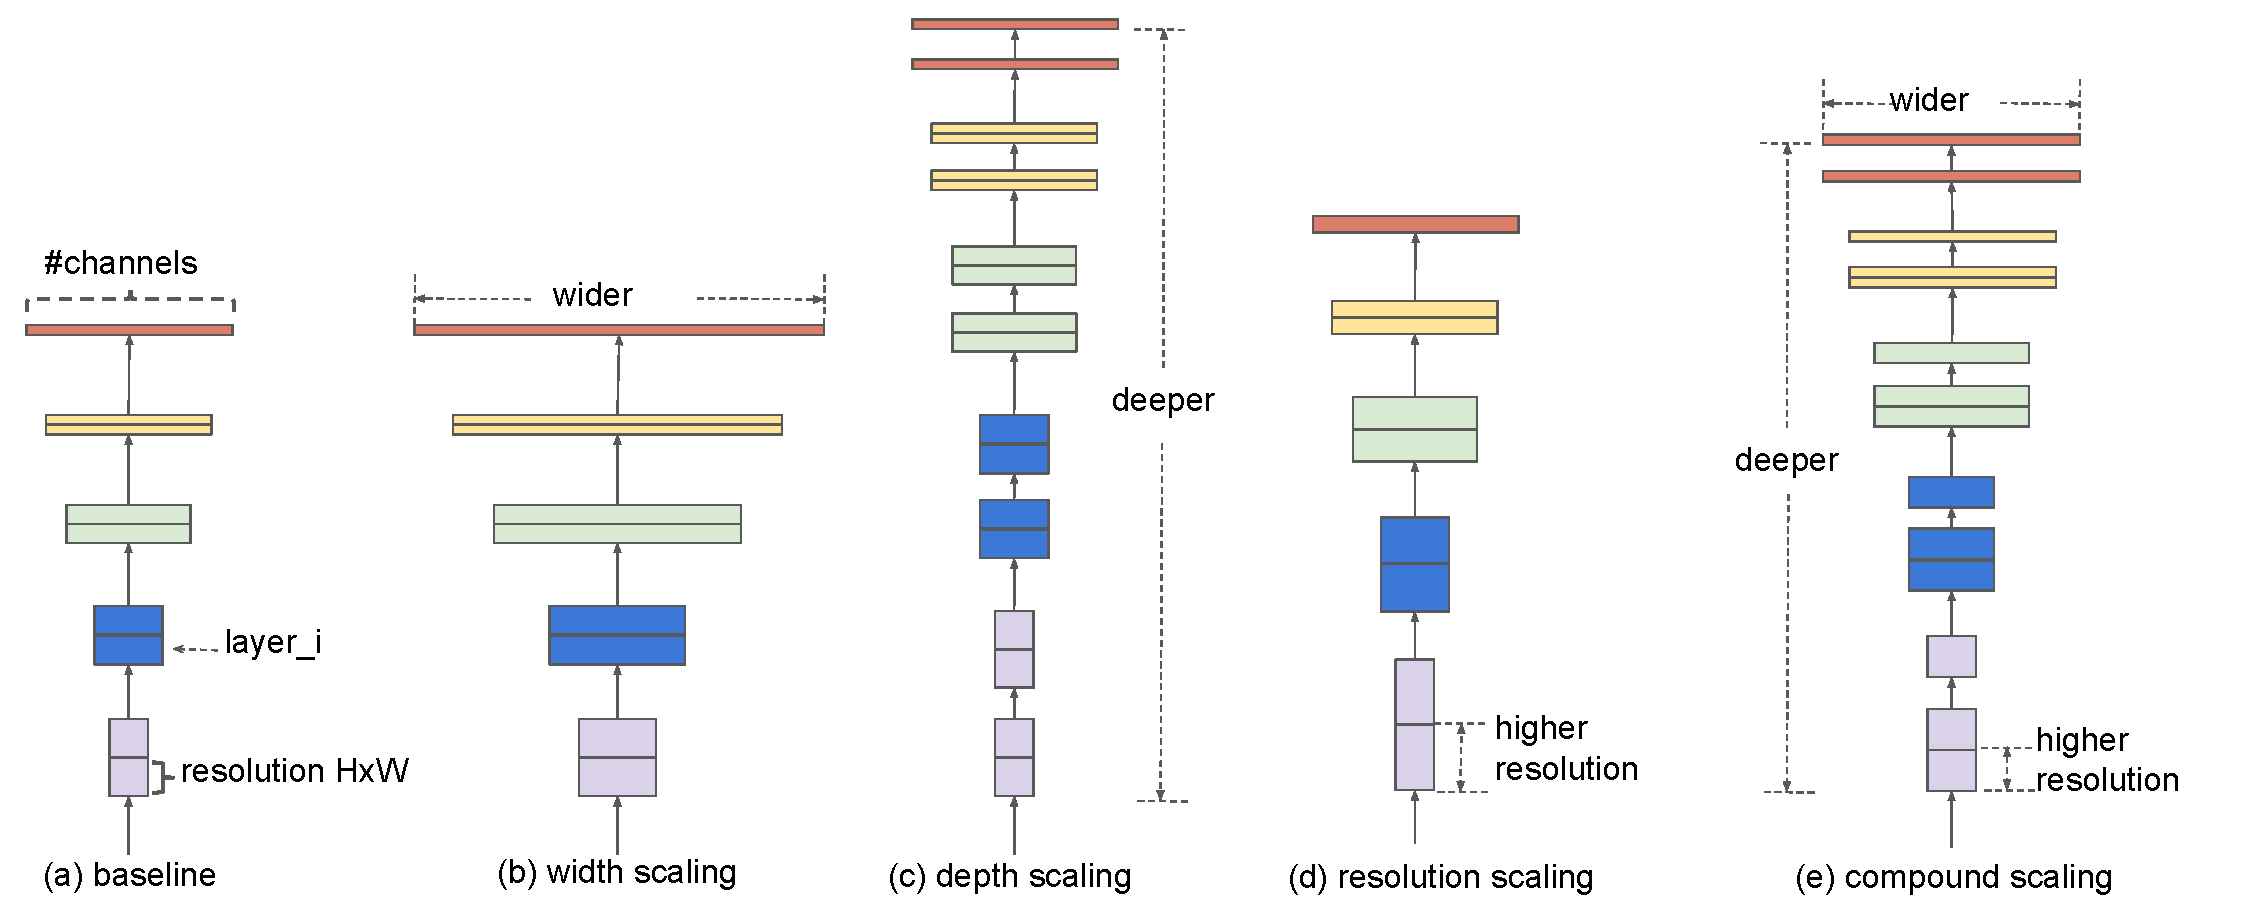
\includegraphics[width=0.80\textwidth]{figures/main/ch3-related_work/scalecompare.pdf}
  \caption{Illustration of the scaling of the EfficientNet architecture.}
  \label{figure:p1-ch3-illustration_efficientnet}
\end{figure}

More recently, \citet{zoph2018learning,real2019regularized} have designed algorithms that automatically tune the width and depth of neural network architectures to obtain the best trade-off between compactness and accuracy.
With this approach, \citet{tan2019efficientnet} found a new compound scaling method that uniformly scales network width and depth leading to efficient and compact architecture.
\Cref{figure:p1-ch3-illustration_efficientnet} illustrates the different scaling proposed by~\citet{tan2019efficientnet}.

% Finally, in the context of deep learning, compact representations have gained much attention over the past years as a way to compress models or to reduce memory requirements.
% In this thesis, we focus on building compact neural networks with structured matrices.
% Hereafter, we present a comprehensive overview of the existing techniques in this line of research.



% --> Compact Neural Networks Architecture

% Without consideration of specific memory representations, data structures or structured linear layers, it is still possible to design compact neural networks.
%
% However, researchers have demonstrated that increasing the width of shallow neural networks increased their performance~\cite{howard2017mobilenets,sandler2018mobilenetv2,tan2019mnasnet,zagoruyko2016wide} due to their capacity to capture more fine-grained features.
% Finally, depth is a common and effective way to scale neural networks and many deep architectures have been proposed~\cite{he2016deep, huang2016deep, szegedy2016rethinking,szegedy2017inception,xiao2018dynamical}. 
% The intuition is that deep neural network can capture richer and more complex features.
%
% After observing that large and deep neural networks outperformed shallow ones \cite{huang2019gpipe,brown2020language} and the observation that a lot of parameters in large neural networks were redundant~\cite{dai2018compressing,frankle2018lottery}, an important question arises: \emph{do neural networks needs to be large \ie, deep and wide, and if not, which architecture provides the best accuracy?} 

% \citet{ba2014deep} tried to answer this question and empirically demonstrated that shallow neural networks can learn the complex functions previously learned by another neural network. 
% This observation was then leveraged by~\citet{hinton2015distilling} for compressing trained neural networks.
% Their technique, called \emph{model distillation}, consists to train a large complex model using all the available data and resources to be as accurate as possible, then a smaller and more compact model is trained to approximate the first model.
% Although, this approach can be interesting for deployment purposes, it is still required to train one large network and one shallow, which entails a significant training cost.
%
% Instead of compressing the model after the training step, researchers still tried to design architectures that are compact by nature but finding the best trade-off between depth, width and performance has proved to be a tedious work.
% In order to scale the search, recent works have devised algorithms to automatically find the best architecture for a specific use case.
% \citet{zoph2018learning,real2019regularized} have tried to tune the wide and depth of neural network architectures to obtain the best trade-off between efficiency and accuracy but these methods required a lot of manual tuning.
% More recently, with a similar method, \citet{tan2019efficientnet} found a new compound scaling method to uniformly scales network width, depth, and resolution leading to groundbreaking result in terms of efficiency and accuracy.




%%%%%%%%%%%%%%%%%%%%%%%%%%%%%%%%%%%%%%%%%%%%%%%%%%%%%%%%%%%%%%%%%%%%%%%%%%%%%%%%
\subsection{Building Compact Neural Networks with Structured Matrices}
\label{subsection:ch3-building_compact_neural_networks_with_structured_matrices}
%%%%%%%%%%%%%%%%%%%%%%%%%%%%%%%%%%%%%%%%%%%%%%%%%%%%%%%%%%%%%%%%%%%%%%%%%%%%%%%%

% An effective method to build compact neural networks is to constrain the hypothesis space in which the learning algorithm ``chooses'' the predictor.
% As seen in \Cref{chapter:ch2-background}, this constraint is called \emph{inductive bias}. 

% Another way of constraining the weight representation and reduce the memory requirement of neural networks is to impose a \emph{structure} on weight matrices. 

% The idea of building compact neural networks with structured matrices consists of replacing the weight matrices $\Wmat^{(i)}$ with \emph{structured matrices}.


% A structured matrix is a $n \times n$ matrix whose entries have a formulaic relationship, allowing the matrix to be represented with fewer than $n^2$ parameters.
% The formulaic relationship between entries is an important feature to consider, for example, a sparse matrix has fewer than $n^2$ parameters but does not have a clear relationship between its entries.

% by using \emph{structured neural networks}. 
% The idea of structured neural networks consists of replacing the dense weight matrices with \emph{structured} ones.

An effective method to build compact neural networks is to constrain the hypothesis space by imposing a \emph{structure} on the weight matrices which constitute the different layers of the network.
% A structured matrix is a $n \times n$ matrix which can be represented with fewer than $n^2$ parameters and where the entries are distributed along specific rules.

%%%%%%%%%%%%%%%%%%%%%%%%%%%%%%%%%%%%%%%%%%%%%%%%%%%%%%%%%%%%%%%%%%%%%%%%%%%%%%%%
\paragraph{Structured Neural Networks with Low Rank Approximation} ~\\
%%%%%%%%%%%%%%%%%%%%%%%%%%%%%%%%%%%%%%%%%%%%%%%%%%%%%%%%%%%%%%%%%%%%%%%%%%%%%%%%

\noindent
For example, \citet{sainath2013lowrank} were among the first to use low-rank matrices in deep learning contexts followed by the work of~\citet{jaderberg2014speeding,yu2017compressing}.
Their work consists in replacing the weight matrices of size $n \times m$ by the product of two rectangular matrices of size $n \times r$ and $r \times m$, where $r$ corresponds to the rank of the new matrix. 
In order to reduce the number of parameters, the rank $r$ is chosen to be small such that $r \ll \min(m, n)$.
By representing the weight matrices with a low-rank decomposition, one can reduce the storage from $mn$ parameters to $(mr + nr)$ and accelerate the matrix-vector product from $\bigO(mn)$ to $\bigO(mr + rn)$.
To enforce the low-rank constraint, reduced storage and computation time during training, the authors trained the coefficients of the two rectangular matrices directly. 
Formally, let $\Wmat \in \Rbb^{n \times m}$ be a weight matrix and let $\widetilde{\Wmat}$ be the low-rank approximation of rank $r$ of the matrix $\Wmat$.
Then, the low-matrix $\widetilde{\Wmat}$ can be decomposed by the product of two rectangular matrices $\Umat \in \Rbb^{n \times r}$ and $\Vmat \in \Rbb^{r \times m}$ such that $\widetilde{\Wmat} = \Umat \Vmat$.
Therefore, a neural network layer with low-rank approximation can be expressed as follows:
\begin{equation}
  \layer_{\Umat, \Vmat, \bvec} (\xvec) = \act\left( \Umat \Vmat \xvec + \bvec \right) .
\end{equation}
The scalar $r$ defining the size of the two rectangular matrices becomes an hyper-parameter and controls the trade-off between the expressivity and compactness of the layer. 

In the same vein, \citet{oseledets2011tensor} have proposed the \emph{Tensor Train decomposition} (TT-decomposition), which is based on the tensor rank decomposition (Tucker decomposition) proposed by~\citet{hitchcock1927expression} and named after \citet{tucker1966some}.
The TT-decomposition is defined as follows.
Let $\boldsymbol{\Aset} \in \Rbb^{n_1 \times n_2 \times \dots \times n_{d-1} \times n_d}$ be a $d$-dimensional tensor.
The Tensor-Train Decomposition factorizes $\boldsymbol{\Aset}$ in a product of third-order tensors and it is given by: 
\begin{equation}
  (\boldsymbol{\Aset})_{(i_1,\dots,i_d)} = (\Gmat^{(1)})_{(i_1, :)} (\boldsymbol{\Gset}^{(2)})_{(:, i_2, :)} (\boldsymbol{\Gset}^{(3)})_{(:, i_3, :)} \dots (\Gmat^{(d)})_{(:, i_d)}
\end{equation}
where $\Gmat^{(i)}$ are matrices and $\boldsymbol{\Gset}^{(i)}$ are third-order tensors of size $r_{i} \times r_{i+1}$ called \emph{TT-cores}.
The sequence $\{r_k\}_{k=0}^d$ is referred to as the ranks of the TT-representation.
The above equation can be equivalently rewritten as a sum of elements of the TT-cores:
\begin{equation}
  (\boldsymbol{\Aset})_{(i_1,\dots,i_d)} = \sum_{\alpha_1, \dots, \alpha_{d-1}} (\Gmat^{(1)})_{(i_1, \alpha_1)} (\boldsymbol{\Gset}^{(2)})_{(\alpha_1, i_2, \alpha_2)} \dots (\Gmat^{(d)})_{(\alpha_{d-1}, i_d)}
\end{equation}
\citet{oseledets2011tensor} have shown that for an arbitrary tensor $\boldsymbol{\Aset}$, several TT-representations exist with different ranks.
The TT-decomposition can be very efficient in terms of memory requirement if the ranks are small.
Indeed, the tensor $\boldsymbol{\Aset}$ has $\prod_{k=1}^{d} n_k$ values compared with $\sum_{k=1}^d n_k r_{k-1} r_k$ values.

The TT-decomposition has been extensively used in the context of deep learning.
\citet{novikov2015tensorizing} was one of the first to use this technique to reduce the number of parameters of neural networks by using the decomposition to replace the fully connected layer of the VGG architecture~\cite{simonyan2014very}.
They reported a compression factor of the dense weight matrix up to 200000 times leading to the compression factor of the whole network up to 7 times with only 0.3 point drop of TOP-5 accuracy on ImageNet~\cite{deng2009imagenet}.
With this work, \citet{novikov2015tensorizing} have demonstrated that the TT-decomposition allows an important reduction of the number of parameters while preserving the expressive power of the layers.
Later, the TT-decomposition was used in other types of architectures.
\citet{garipov16ttconv} used it to compress convolutional layers as well as fully connected layers.
\citet{yang2017tensor} used it in the context of video classification, \citet{tjandra2017compressing} compressed the layers of recurrent neural networks and finally, \citet{xindian2019tensorized} developed a compact architecture based on TT-decomposition for Language Modeling.

However, the Tensor-Train decomposition has some limitations.
Although it can reduce the number of parameters when the ranks are low, finding the best alignment of the tensor dimensions in order to find the best optimized TT-cores remains a challenging problem, as stated by~\citet{pan2019compressing}.


% In the same vein, \citet{novikov2015tensorizing} have proposed a generalization of low-rank decomposition.
% Instead of searching for low-rank approximation of the weight matrices, they consider multi-dimensional tensors and apply the \emph{Tensor Train decomposition} algorithm \cite{oseledets2011tensor}.
% The Tensor Train decomposition allows an important reduction of the number of parameters while preserving the expressive power of the layers.



%%%%%%%%%%%%%%%%%%%%%%%%%%%%%%%%%%%%%%%%%%%%%%%%%%%%%%%%%%%%%%%%%%%%%%%%%%%%%%%%
\paragraph{Neural Networks with Diagonal and Circulant Matrices} ~\\
%%%%%%%%%%%%%%%%%%%%%%%%%%%%%%%%%%%%%%%%%%%%%%%%%%%%%%%%%%%%%%%%%%%%%%%%%%%%%%%%

\noindent

% Since the seminal work of \citet{ailon2009fast}, structured transforms have been extensively studied in the context of dimensionality reduction and random projections.
% For example, the Fastfood transform which was proposed by \cite{le2013fastfood}  
%
% Other types of structured transforms have been used to  


% The authors have replaced dense matrices of fully connected layers with adaptive structured matrices of the form: $\Smat\Hmat\Gmat\mathbf{\Pi}\Hmat\Bmat$ where $\Smat$, $\Gmat$, and $\Bmat$ are adaptive diagonal matrices, $\mathbf{\Pi}$ is a random permutation matrix, and $\Hmat$ is the Walsh-Hadamard matrix.


% Other types of decomposition have been used to reduce the number of parameters of neural networks.
% The Fastfood transform which was originally used for approximating kernel expansions~\cite{le2013fastfood}, was later used in neural networks by~\citet{yang2015deep} leading to the Deep Fried Convnets architecture.
% The authors have replaced dense matrices of fully connected layers with adaptive structured matrices of the form: $\Smat\Hmat\Gmat\mathbf{\Pi}\Hmat\Bmat$ where $\Smat$, $\Gmat$, and $\Bmat$ are adaptive diagonal matrices, $\mathbf{\Pi}$ is a random permutation matrix, and $\Hmat$ is the Walsh-Hadamard matrix.
% Later, the \emph{Structured Spinners} transform of the form: $\Hmat\Dmat^{(3)} \Hmat\Dmat^{(2)} \Hmat\Dmat^{(1)}$, where $\Hmat$ is the Walsh-Hadamard matrix, and $\Dmat^{(i)}$ for $i \in {1, 2, 3}$ is a random $\pm1$-diagonal matrix, was originally proposed by~\citet{andoni2015practical} and used in deep learning settings by~\citet{bojarski2017structured}.



% Key to Fastfood is the observation that Hadamard 
% matrices when combined with diagonal Gaussian
% matrices exhibit properties similar to dense
% Gaussian random matrices. Yet unlike the
% latter, Hadamard and diagonal matrices are
% inexpensive to multiply and store.

% which can be viewed as a generalized class of Fourier transforms.

% Decomposition with structured matrices of interest for the contributions of this thesis are the ones based on diagonal and circulant matrices.

% More practically, \citet{hinrichs2011johnson} have shown that the \DC transform $\xvec \mapsto \Dmat \Cmat \xvec$, where the matrix $\Dmat$ is a diagonal matrix with entries sampled from $\{1, -1\}$ and $\Cmat$ is a circulant matrix based on a sequence of independent identically distributed random variables respect the \citeauthor{johnson1984extensions} lemma.
\citet{cheng2015exploration} proposed to replace the weight matrix of a fully connected layer by the product of a circulant and a diagonal matrix leading to following structured layer:
\begin{equation}
  \layer_{\Dmat, \Cmat, \bvec} (\xvec) = \act \left( \Dmat \Cmat \xvec + \bvec \right) \enspace,
\end{equation}
where the circulant matrix is learned by a gradient-based optimization algorithm and the diagonal matrix entries are sampled at random in $\{-1, 1\}$. 
The idea of replacing dense matrices with circulant ones comes from their use in dimensionality reduction with the \emph{fast Johnson-Lindenstrauss transform}~\cite{hinrichs2011johnson,vybiral2011variant}, binary embedding~\cite{yu2014circulant}, and kernel approximation~\cite{yu2015compact}, etc.
Circulant matrices exhibit several interesting properties from the perspective of numerical computations.
Recall from \Cref{theorem:ch2-diagonalization_circulant_matrix} that circulant matrices can be diagonalized with the Fourier Transform as follows:
\begin{equation}
  \Cmat = \frac{1}{n} \Umat_n^* \diag(\Umat_n \cvec) \Umat_n \enspace.
\end{equation}
where the vector $\cvec$ corresponds to the first columns of the matrix $\Cmat$.
This decomposition allows a compact representation in memory ($n$ values instead of $n^2$) and efficient matrix-vector product with the FFT algorithm (see \Cref{algorithm:ch2-matrix_vector_product_circulant_matrix}).
% Thanks to this decomposition, circulant matrices exhibit several interesting properties from the perspective of numerical computations. Most importantly, any $n \times n$ circulant matrix $\Cmat$ can be represented using only $n$ coefficients instead of the $n^2$ coefficients required to represent classical unstructured. In addition, the matrix-vector product is simplified from O(n 2) to O(n log(n)) using the convolution theorem.
% Thanks to this decomposition, circulant matrices offer a compact representation in memory (they can be expressed with only $n$ values instead of $n^2$) and an efficient matrix-vector product with the FFT algorithm (see \Cref{algorithm:ch2-matrix_vector_product_circulant_matrix}).
Despite the reduction of expressivity, \citet{cheng2015exploration} demonstrated good empirical results using only a fraction of the original weights (90\% reduction). 


\citet{moczulski2016acdc} built upon the work of~\citet{cheng2015exploration} and \citet{huhtanen2015factoring} and introduced two \emph{Structured Efficient Linear Layers} (SELL) based on the Fourier and cosine transforms.
First, by observing that the DC transform cannot express an arbitrary linear operator they proposed to apply the result of \citet{huhtanen2015factoring} which states that almost all matrices can be decomposed as a product of DC transforms.
\begin{theorem}[Reformulation from \citet{huhtanen2015factoring}] \label{theorem:ch3-huhtanen}
  For every matrix $\Mmat \in \Cbb^{n \times n}$, for any $\epsilon > 0$, there exists a sequence of matrices $\{ \Amat^{(i)} \}_{i \in [2n-1]}$ where $\Amat^{(i)}$ is a circulant matrix if $i$ is odd, and a diagonal matrix otherwise, such that $\norm{\Amat^{(1)} \ldots \Amat^{(2n-1)} - \Mmat} < \epsilon$.
\end{theorem}
\noindent
Based on this result, they proposed to parameterize the layers of a neural network with $k$ products of diagonal and circulant matrices as follows:
\begin{equation} \label{equation:acdc_layer}
  \layer_{\Dmat, \Cmat, \bvec} (\xvec) = \act \left( \left(\prod_{i = 1}^{k} \Dmat^{(i)} \Cmat^{(i)} \right) \xvec + \bvec \right)
\end{equation}
where $\Dmat$ and $\Cmat$ are sequences of $k$ diagonal and circulant matrices respectively.
This structured layer is therefore parameterized by $n(2k+1)$ values and the value $k$ becomes a hyper-parameter controlling the trade-off between compactness and expressivity. 
By diagonalizing the circulant matrix, the layer in \Cref{equation:acdc_layer} can be expressed as a product of diagonal matrices and the Fourier transform as follows:
\begin{equation} \label{equation:ch3-laye_acdc}
  \layer^\act_{\dvec, \cvec, \bvec} (\xvec) = \act \left(\frac{1}{n^k} \left(\prod_{i = 1}^{k} \diag\left(\dvec^{(i)}\right) \Umat_n^* \diag\left(\Umat_n \cvec^{(i)}\right) \Umat_n \right) \xvec + \bvec \right)
\end{equation}
\noindent
Although interesting and demonstrating good empirical results, the work of~\citet{moczulski2016acdc} suffers from multiple limitations. 
First, the result from~\citet{huhtanen2015factoring} is expressed with respect to $n$, the size of the matrices $\Amat$.
Therefore, the theorem does not provide any insights regarding the expressive power of $k$ factors when $k$ is much lower than $2n-1$ as it is the case in most practical scenarios they consider.
Finally, in order to stay in the real domain, they replaced the Fourier transform in~\Cref{equation:ch3-laye_acdc} with the cosine transform thus learning a different kind of linear transform (see the work of~\citet{sanchez1995diagonalizing} which characterizes the matrices diagonalizable by the cosine transform).
Furthermore, because the cosine transform does not diagonalize circulant matrices, \Cref{theorem:ch3-huhtanen} no longer applies.


% \vspace{0.3cm}

%%%%%%%%%%%%%%%%%%%%%%%%%%%%%%%%%%%%%%%%%%%%%%%%%%%%%%%%%%%%%%%%%%%%%%%%%%%%%%%%
\paragraph{General Representation of Structured Linear Maps: LDR and K-Matrices} ~\\
%%%%%%%%%%%%%%%%%%%%%%%%%%%%%%%%%%%%%%%%%%%%%%%%%%%%%%%%%%%%%%%%%%%%%%%%%%%%%%%%

\vspace{-0.5cm}

General framework for structured matrices that reduce the memory footprint but also accelerate matrix-vector product operations have been used to build compact neural networks.
\citet{sindhwani2015structured} have used the notion of low displacement rank presented in \Cref{subsection:ch2-general_frameworks_for_structured_matrices} to learn a broad family of structured matrices.
Recall from~\Cref{theorem:ch2-toeplitz_like} that all matrices expressed as the following sum of products are called \emph{Toeplitz-like} matrices:
\begin{equation}
    \Mmat = \sum_{j=1}^{r} \Zmat_1(\gvec^{(j)}) \Zmat_{-1}(\Jmat_n \hvec^{(j)})
\end{equation}
where $\Zmat_f$ is an $f$-circulant matrix defined in \Cref{definition:ch2-f_circulant_matrix} and $\Gmat = \leftmat \gvec^{(1)} \ldots \gvec^{(r)} \rightmat, \Hmat = \leftmat \hvec^{(1)} \ldots \hvec^{(r)} \rightmat \in \Rbb^{n \times r}$ with $r \ll n$.
More precisely, \citet{sindhwani2015structured} proposed to learn Toeplitz-like matrices by learning the factors $\Gmat$ and $\Hmat$. 
Therefore, they proposed the following parameterized layer:
\begin{equation}
  \layer_{\Gmat, \Hmat, \bvec}(\xvec) = \act \left( \left(\sum_{j=1}^{r} \Zmat_1\left(\gvec^{(j)}\right) \Zmat_{-1}\left(\Jmat_n \hvec^{(j)}\right) \right) \xvec + \bvec \right)
\end{equation}
where the rank $r$ is a hyper-parameter and controls the number of parameters of the layer.
In addition to offer fast matrix-vector product, they have showed that this class of layers is very rich from a modeling perspective.
More precisely, they characterize the expressivity of the layer as follows: 
\begin{theorem}[LDR expressivity \citet{pan2001structured,sindhwani2015structured}] ~\\
  The set of all $n \times n$ matrices that can be written as, $\sum_{i=1}^{r} \Zmat_1(\gvec^{(i)}) \Zmat_{-1}(\hvec^{(i)})$
  for some $\Gmat = \leftmat \gvec^{(1)} \ldots \gvec^{(r)} \rightmat,
  \Hmat = \leftmat \hvec^{(1)} \ldots \hvec^{(r)} \rightmat \in \Rbb^{n \times r}$ contains:
  \begin{compactitem}
    \item All $n \times n$ Circulant and Skew-Circulant matrices for $r \geq 1$.
    \item All $n \times n$ Toeplitz matrices for $r \geq 2$.
    \item Inverses of Toeplitz matrices for $r \geq 2$.
    \item All products of the form $\Amat^{(1)} \ldots \Amat^{(t)}$ for any $t \leq \frac{r}{2}$.
    \item All linear combinations of the form $\sum_{i=1}^p \beta_i \Amat^{(1, i)} \ldots \Amat^{(t, i)}$ for any $t \leq \frac{r}{2p}$.
    \item All $n\times n$ matrices for $r=n$.
  \end{compactitem}
  where each $\Amat^{(i)}$ above is a Toeplitz matrix or the inverse of a Toeplitz matrix. 
\end{theorem}
\noindent

In the same line of work, \citet{thomas2018learning} have proposed neural network layers directly form the Krylov decomposition presented in~\Cref{theorem:ch2-krylov_decomposition} which encompasses an even larger family of structured matrices including Toeplitz-like, Vandermonde-like, Cauchy-like ones.
Despite being elegant and general, we found that the LDR framework suffers from several limits which are inherent to its generality and makes it difficult to use in the context of deep neural networks.
% First, the training procedure for learning LDR matrices is highly involved and implies many complex mathematical objects such as Krylov matrices.
As acknowledged by the authors, the number of parameters required to represent a given structured matrix (a Toeplitz matrix) in practice is unnecessarily high (higher than required in theory) making the training very hard. 



More recently, another type of generalization of structured linear maps has been proposed by~\citet{dao2019learning,dao2020kaleidoscope}.
They introduced a family of matrices called \emph{kaleidoscope matrices} (K-matrices) which are the product of sparse matrices with specific predefined sparsity patterns.
They showed that this type of matrices can capture any sparse matrix with near-optimal space (parameter) and time (arithmetic operation) complexity.
The authors claim that their structured linear maps can capture more common structures with a few numbers of parameters than the displacement operators presented above.
More precisely, their representation is based on products of a particular building block known as a butterfly matrix introduced by~\citet{parker1995random}.
Butterfly matrices have been extensively used in numerical linear algebra~\cite{parker1995random,li2015butterfly} and machine learning~\cite{mathieu2014fast,jing2017tunable,munkhoeva2018quadrature,dao2019learning,choromanski2019unifying}.







%%%%%%%%%%%%%%%%%%%%%%%%%%%%%%%%%%%%%%%%%%%%%%%%%%%%%%%%%%%%%%%%%%%%%%%%%%%%%%%%
\section{Related Work on Lipschitz Regularization}
\label{section:ch3-related_work_on_lipschitz_regularization}
%%%%%%%%%%%%%%%%%%%%%%%%%%%%%%%%%%%%%%%%%%%%%%%%%%%%%%%%%%%%%%%%%%%%%%%%%%%%%%%%

%%%%%%%%%%%%%%%%%%%%%%%%%%%%%%%%%%%%%%%%%%%%%%%%%%%%%%%%%%%%%%%%%%%%%%%%%%%%%%%%
\subsection{The Global Lipschitz Constant of Neural Networks}
\label{subsection:ch3-the_global_lipschitz_constant_of_neural_networks}
%%%%%%%%%%%%%%%%%%%%%%%%%%%%%%%%%%%%%%%%%%%%%%%%%%%%%%%%%%%%%%%%%%%%%%%%%%%%%%%%

\noindent
The regularization of the Lipschitz constant of neural networks has seen a growing interest in the training of neural networks.
Indeed, numerous results have shown that neural networks with a low Lipschitz constant exhibit better generalization~\cite{bartlett2017spectrally} and higher robustness to adversarial attacks~\cite{szegedy2013intriguing,tsuzuku2018lipschitz, farnia2018generalizable}.

The Lipschitz constant, defined in~\Cref{definition:ch2-lipschitz_constant}, is a measure of the stability of the network
If the Lipschitz constant is high, the network will tend to be more sensitive to input perturbation.
Intuitively, the Lipschitz constant $k$ of a function $f$ is a bound on the slope of $f$.
Meaning, if the input changes by $\epsilon$, the output changes by at most $k\epsilon$.
Therefore, the Lipschitz constant of a function can also be expressed using the differential operator as follows:
\begin{theorem}[Rademacher's Theorem] \label{theorem:ch3-lipschitz_differential_op}
  If $f: \Rbb^n \rightarrow \Rbb^m$ is a Lipschitz continuous function, then $f$ is differentiable almost everywhere.
  Moreover, if $f$ is Lipschitz continuous, then
  \begin{align}
    \lip{f} = \sup_{\xvec \in \Rbb^n} \norm{\mathrm{D}_\xvec f(\xvec)}_2
  \end{align}
  where $\mathrm{D}_\xvec$ is the differential operator of $f$ at $\xvec$.
\end{theorem}

\citet{tsuzuku2018lipschitz} have studied the relationship between the robustness of a neural network and the Lipschitz constant and the margin of the neural networks. 
By the definition of the Lipschitz constant, we have the following:
\begin{equation}
  \norm{N(\xvec) - N(\xvec + \adv)}_2 \leq \lip{N} \norm{\adv}_2
\end{equation}
Recall the margin operator $\Mset: \Rbb^k \times [k] \rightarrow \Rbb$ from~\Cref{subsection:ch2-recent_results_on_the_theory_of_neural_networks} defined as:
\begin{equation}
  \Mset(\vvec, j) \triangleq \vvec_j - \max_{i \neq j} \vvec_i
\end{equation}
% Let us denote the margin of the neural network $N$ with respect to the tuple $(\xvec, y)$ as follows:
% \begin{equation}
%   \mathcal{M}^{N}_{(\xvec, y)} \triangleq N(\xvec)_y - \max_{i \neq y} \left( N(\xvec) \right)_i
% \end{equation}
Then, we have the following proposition which characterize the robustness of a neural network with respect to its margin and Lipschitz constant.
\begin{proposition}[\citet{tsuzuku2018lipschitz}]
  \begin{equation} \label{equation:ch3-margin_guarded_area}
    \Mset \big( N(\xvec), y \big) \geq \sqrt{2} \lip{N} \norm{\adv}_2 \quad \Longrightarrow \quad \Mset \big( N(\xvec + \adv), y \big) \geq 0
  \end{equation}
  \removespace
\end{proposition}
\noindent
If the inequality on the right-hand side of \Cref{equation:ch3-margin_guarded_area} is verified then the adversarial margin is positive, \ie, the network correctly predicts the label. 
From this proposition, we can conclude that for a given neural network with specific margins, a lower Lipschitz constant allows for an increase in robustness. 
Note that the margin is already maximized in a multi-class setting with the cross-entropy loss as stated in~\citet{hein2017formal}.
A multitude of work have tried to reduce the Lipschitz constant in order to improve adversarial robustness.
However, \citet{scaman2018lipschitz} have shown that computing the exact Lipschitz constant of a neural network is NP-hard.
The following theorem shows that, even for shallow neural network, exact Lipschitz computation is not achievable in polynomial time:
\begin{theorem}[\citet{scaman2018lipschitz}] \label{theorem:ch3-lipschitz_computation}
  Let us define the problem associated with the exact computation of the Lipschitz constant of a $2$-layer neural network with $\relu$ activation:
  \begin{itemize}%[topsep=0pt,noitemsep]
    \item[] \textbf{Input:} Two matrices $\Wmat^{(1)} \in \Rbb^{l \times n}$ and $\Wmat^{(2)} \in \Rbb^{m \times l}$, and a constant $c \geq 0$.
    \item[] \textbf{Question:} Let $N = \Wmat^{(2)} \circ \rho \circ \Wmat^{(1)}$ where $\rho$ is the $\relu$ activation function. \emph{Is the Lipschitz constant $\lip{N} \leq c$ ?}
  \end{itemize}
  Then, assuming that $\mathbf{P} \neq \mathbf{NP}$, the problem above is \textbf{NP}-hard. 
\end{theorem}


\noindent
To overcome this difficulty, researchers have relied on devising a tight upper bound of the Lipschitz constant.
For example, \citet{scaman2018lipschitz} have shown that the Lipschitz constant of a neural network $N$ can be explicitly formulated using \Cref{theorem:ch3-lipschitz_differential_op} and the chain rule:
\begin{equation} \label{equation:ch3-decomposition_jacobian_lipschitz}
  \lip{\nn} = \sup_{x \in \Rbb^n} \norm{\Wmat^{(p)} \diag(\rho'_\depth(\theta_\depth)) \dots \Wmat^{(2)} \diag(\rho'_1(\theta_1)) \Wmat^{(1)}}_2,
\end{equation}
where $\theta_i = \layer^{\act_i}_{\Wmat^{(i)}, \bvec^{(i)}} \circ \cdots \circ \layer^{\act_1}_{\Wmat^{(1)}, \bvec^{(1)}}(\xvec)$ is the intermediate output after $i$ layers.
The Lipschitz of the neural network $N$ can then be upper bounded as follows:
\begin{align}
  \lip{\nn} &\leq \max_{\forall i,\ \sigma_i \in [0, 1]^{w^{(i+1)}}} \norm{\Wmat^{(\depth)} \diag(\sigma_{\depth-1}) \dots \diag(\sigma_1) \Wmat^{(1)}}_2 \notag \\
  &\leq \max_{\forall i,\ \sigma_i \in [0, 1]^{w^{(i+1)}}} \norm{ \pmb{\Sigma}^{(\depth)} \Vmat^{(\depth)\top} \diag(\sigma_{\depth-1}) \dots \diag(\sigma_1) \Umat^{(1)} \pmb{\Sigma}^{(1)}}_2 \notag \\
  &\leq \prod_{i=1}^{\depth-1} \max_{\sigma_i \in [0, 1]^{w^{(i+1)}}} \norm{\widetilde{\pmb{\Sigma}}^{(i+1)} \Vmat^{(i+1)\top} \diag(\sigma_{i+1}) \Umat^{(i)} \widetilde{\pmb{\Sigma}}^{(i)}}_2 
\end{align}
where $\widetilde{\pmb{\Sigma}}^{(i)} = \pmb{\Sigma}^{(i)}$ if $i \in \{1, \depth\}$ and $\widetilde{\pmb{\Sigma}}^{(i)} = {\pmb{\Sigma}^{(i)}}^{1/2}$ otherwise.
The first inequality is due to the fact that the derivatives of the activation functions are bounded, \ie, $\rho_i(\xvec) \in [0, 1]^{w^{(i+1)}}$, the second inequality is obtained by decomposing each weight matrix $\Wmat^{(i)}$ with the \emph{Singular Value Decomposition} such that $\Wmat^{(i)} = \Umat^{(i)} \pmb{\Sigma}^{(i)} \Vmat^{(i)\top}$; and finally, the last inequality is due to the submultiplicativity of the operator norm.
Although accurate, this bound is still computationally expensive to compute due to the singular value decomposition and the optimization for each layer. 
In the same line of research, recent work~\cite{fazlyab2019safety,fazlyab2019efficient,latorre2020lipschitz} has proposed a tight bound on the Lipschitz constant of the full network with the use of semi-definite programming.
More precisely, \citet{fazlyab2019efficient} have demonstrated the following result:
\begin{theorem}[Lipschitz bounds \citet{fazlyab2019efficient}] \label{theorem:ch3-lipschite_semidefinite_programming}
  Consider a neural network $N: \Rbb^n \rightarrow \Rbb^m$ such that $N(\xvec) = \Wmat^{(2)} \rho(\Wmat^{(1)} \xvec + \bvec^{(1)}) + \bvec^{(2)}$.
  Suppose the activation function $\rho$ is \emph{slope-restricted} in the sector $[\alpha,\beta]$, more precisely:
  \begin{equation}
    \alpha \leq \frac{\rho(y) - \rho(x)}{y-x} \leq \beta \quad \forall x,y \in \Rbb. 
  \end{equation}
  Define the set $\mathcal{T}_{n}$ as the following:
  \begin{equation*}
    \mathcal{T}_n = \{\Tmat \in \Sbb^n \mid \Tmat = \sum_{i=1}^{n} \lambda_{ii} \evec^{(i)} \evec^{(i)\top} + \sum_{1 \leq i<j \leq n} \lambda_{ij}(\evec^{(i)} - \evec^{(j)})(\evec^{(i)}-\evec^{(j)})^\top, \lambda_{ij} \geq 0 \}.
  \end{equation*}
  where $\Sbb^d$ is the set of all symmetric matrices of size $n \times n$.
  Suppose there exists a constant $c>0$ such that the matrix inequality
  \begin{align}
    \Mmat(c,\Tmat) \triangleq
      \leftmatrix
      -2\alpha \beta \Wmat^{(1)\top} \Tmat \Wmat^{(1)} - c \Imat_n & (\alpha+\beta) \Wmat^{(1)\top} \Tmat  \\
      (\alpha+\beta) \Tmat \Wmat^{(1)} & -2\Tmat+\Wmat^{(2)\top} \Wmat^{(2)}
      \rightmatrix
      \leq 0,
  \end{align}
  holds for some $\Tmat \in \mathcal{T}_{n}$. Then $\norm{N(\xvec)-N(\yvec)}_2 \leq \sqrt{c} \norm{\xvec-\yvec}_2$ for all  $\xvec,\yvec \in \Rbb^n$.
\end{theorem}
\noindent
From \Cref{theorem:ch3-lipschite_semidefinite_programming}, the constant $c$ is an upper bound on the Lipschitz constant of the network.
The authors proposed to find the tightest bound by solving the following optimization problem (Semidefinite Program):
\begin{align}
  \textrm{minimize} \quad c \quad \text{ subject to} \quad \Mmat(c,\Tmat) \leq 0 \quad \text{and} \quad \Tmat \in \mathcal{T}_{n},
\end{align}
where the decision variables are $(c,\Tmat) \in \Rbb_+ \times \mathcal{T}_n$.
Note that $\Mmat(c,\Tmat)$ is linear in $c$ and $\Tmat$ and the set $\mathcal{T}_n$ is convex.
Although, these works on devising a global bound on the Lipschitz constant of a neural network are theoretically interesting, they lack scalability, they can only be computed on small networks and cannot be used during the training of large neural networks for regularization purposes.


%%%%%%%%%%%%%%%%%%%%%%%%%%%%%%%%%%%%%%%%%%%%%%%%%%%%%%%%%%%%%%%%%%%%%%%%%%%%%%%%
\subsection{Lipschitz Constant of Individual Layers}
\label{subsection:ch3-lipschitz_constant_of_individual_layers}
%%%%%%%%%%%%%%%%%%%%%%%%%%%%%%%%%%%%%%%%%%%%%%%%%%%%%%%%%%%%%%%%%%%%%%%%%%%%%%%%

\noindent
% In order to constrain the Lipschitz constant of neural networks, 
Instead of regularizing using the global Lipschitz constant, researchers have devised techniques to reduce the Lipschitz constant of \emph{individual layers} instead. 
The global Lipschitz of a neural network can easily be upper bound by the product of the spectral norm of each weight matrix as follows:
\begin{proposition}[\citet{scaman2018lipschitz}] \label{proposition:ch3-naive_upper_bound_lipschitz}
  Let $N$ be a neural network of $\depth$ layers with 1-Lipschitz activation functions (\eg ReLU,
  Leaky ReLU, Tanh, Sigmoid, etc.), then, the Lipschitz constant of the neural network can be upper bounded as follows:
  \begin{equation} \label{equation:ch3-naive_upper_bound_lipschitz}
    \lip{N} \leq \prod_{i=1}^\depth \norm{\Wmat^{(i)}}_2 \enspace,
  \end{equation}
  where $\Wmat^{(i)}$ are the weights matrices of the neural network.
\end{proposition}

\begin{remark}
  The Lipschitz constant of a layer $\layer_{\Wmat, \bvec}^\rho$ (with a 1-Lipschitz activation function) is equal to the spectral norm of the matrix $\Wmat$ (largest singular value).
  Let $\layer_{\Wmat, \bvec}^\rho: \Rbb^n \rightarrow \Rbb^m$ such that $\layer_{\Wmat, \bvec}^\rho = \rho(\Wmat \xvec + \bvec)$ then by definition of the Lipschitz constant (see \Cref{definition:ch2-lipschitz_constant}) and of the operator norm, we have:
  \begin{equation}
    \lip{\layer_{\Wmat, \bvec}^\rho} = \sup_{\substack{\xvec \in \Rbb^n \\ \xvec \neq 0}} \frac{\norm{\Wmat \xvec}_2}{\norm{\xvec}_2} = \norm{\Wmat}_2
  \end{equation}
  \removespace
\end{remark}

The trivial bound given by the product of layer-wise Lipschitz constants in \Cref{equation:ch3-naive_upper_bound_lipschitz} is known to be loose and pessimistic~\citet{combettes2019lipschitz}.
Furthermore, we can show that reducing the Lipschitz constant of each layer independently does not imply that the global Lipschitz constant of the network will be reduced. 
\begin{proposition} \label{proposition:ch3-limit_bound_lipschitz}
  Let $N_1(\xvec) = \Amat^{(2)} \rho(\Amat^{(1)} \xvec)$ and $N_2(\xvec) = \Bmat^{(2)} \rho(\Bmat^{(1)} \xvec)$ where $\rho$ is the $\relu$ activation function, then $\norm{\Amat^{(1)}}_2 \leq \norm{\Bmat^{(1)}}_2$ and $\norm{\Amat^{(2)}}_2 \leq \norm{\Bmat^{(1)}}_2$, does not imply that $\lip{N_1} \leq \lip{N_2}$.
\end{proposition}
\begin{proof}[\Cref{proposition:ch3-limit_bound_lipschitz}]
  Let
  \begin{align*}
    \Amat^{(1)} &= \leftmatrix 
      \phantom{+}0 & -1 \\ -1 & \phantom{+}0
    \rightmatrix \quad
    \Amat^{(2)}  = \leftmatrix
      -1 & -1 \\ -1 & \phantom{+}0
    \rightmatrix \\
    \Bmat^{(1)} &= \leftmatrix
      \phantom{+}0 & \phantom{+}0 \\ \phantom{+}0 & -1
    \rightmatrix \quad
    \Bmat^{(2)} = \leftmatrix
      -1 & -1 \\ -1 & -1
    \rightmatrix
  \end{align*}
  then: \vspace{-0.5cm}
  \begin{equation*}
    \norm{\Amat^{(1)}}_2 = 1,\ \norm{\Amat^{(2)}}_2 = \sqrt{2}
    \quad \text{and} \quad
    \norm{\Bmat^{(1)}}_2 = 1,\ \norm{\Bmat^{(2)}}_2 = 2
  \end{equation*}
  From \Cref{theorem:ch3-lipschitz_differential_op} and the chain rule, the Lipschitz constant of the networks $N_1$ and $N_2$ can be expressed as follows:
  \begin{align*}
    \lip{N_1} &= \sup_{\xvec \in [0, 1]^2} \norm{\Amat^{(2)} \diag\left(\xvec\right) \Amat^{(1)}}_2 \\
    \lip{N_2} &= \sup_{\xvec \in [0, 1]^2} \norm{\Bmat^{(2)} \diag\left(\xvec\right) \Bmat^{(1)}}_2
  \end{align*}
  It is easy to verify that:
  \begin{equation*}
    \lip{N_1} = \frac{1 + \sqrt{5}}{2} \approx 1.618 \quad \text{and} \quad \lip{N_2} = \sqrt{2} \approx 1.414
  \end{equation*}
  which concludes the proof.
\end{proof}
\noindent
While we cannot have a guarantee that the global Lipschitz will be reduced, we could still have an idea of the value of the global Lipschitz with the upper bound presented in~\Cref{equation:ch3-naive_upper_bound_lipschitz}.


\citet{huster2018limitations} have demonstrated several limitations on the expressive power of neural networks where the product of layer-wise Lipschitz constants is constrained.
In the same vein, \citet{couellan2019coupling} empirically showed that Lipschitz Regularization offers a trade-off between adversarial robustness and expressivity of the network.
However, the bound in \Cref{equation:ch3-naive_upper_bound_lipschitz} appears in multiple generalization bound~\cite{neyshabur2017,bartlett2017spectrally,golowich2018} and adversarial generalization~\cite{farnia2018generalizable} (see \Cref{chapter:ch2-background}) which could suggest that reducing the bound would improve the generalization capabilities of neural networks and its robustness.

Based on this theoretical insight, researchers have developed several techniques to constraint the Lipschitz constant of each layer in order to improve the generalization and robustness of neural networks.
A technique to enforce 1-Lipschitz layers is to impose or promote an orthogonality constraint on the weight matrices.
A square orthogonal matrix $\Mmat$ is a matrix whose columns and rows are orthogonal unit vectors and all eigenvalues are equal to 1.
\citet{cisse2017parseval} and more recently \citet{wang2020orthogonal,huang2020controllable} have proposed to minimize the following term:
\begin{equation} \label{equation:ch3-orthogonality_constraint}
  \frac{\beta}{2} \norm{\Wmat^\top \Wmat - \Imat}_2  \enspace, 
\end{equation}
to promote the orthogonality constraint, in addition to the usual loss function:
In the above equation, the hyper-parameter $\beta$ controls the constraint.
A higher $\beta$ would lead to a better orthogonality constraint and therefore, a Lipschitz constant ``almost'' equal to 1 for all the layers.

On the other hand, \citet{anil2019sorting} proposed to enforce the orthogonality of weight matrices by directly optimizing on the Stiefel
manifold (\ie, the manifold of orthogonal matrices, see~\citet{absil2009optimization}).
To perform this optimization, they made use of an iterative algorithm first introduced by~\citet{bjorck1971iterative}.
For a given matrix $\Wmat = \Wmat^{(0)}$, the algorithm finds the closest orthonormal matrix by computing the following term:
\begin{equation}
  \Wmat^{(k+1)} = \Wmat^{(k)} \left( \Imat + \frac{1}{2} \Vmat^{(k)} + \cdots + (-1)^r {-\frac{1}{2} \choose r}  \left(\Vmat^{(k)}\right)^r \right)
\end{equation}
where $\Vmat = \Imat - \Wmat^{(k)\top} \Wmat^{(k)}$.
Although this algorithm works well on dense matrices, it can be difficult to apply it to convolutions. 
\citet{li2019preventing} built upon this idea and proposed an algorithm to enforce the orthogonality of convolutional layers.
They used the orthogonal projection proposed by \citet{kautsky1994matrix} and \citet{xiao2018dynamical} to build convolutional neural networks with orthogonal convolutions.

All techniques that impose an orthogonality constraint of the weights matrices successfully reduce the Lipschitz constant of the layers of the networks.
Moreover, when the Lipschitz constant of all the layers are low, we could have an idea of the value of the global Lipschitz with the upper bound of~\Cref{equation:ch3-naive_upper_bound_lipschitz} (\ie, if Lipschitz constant of all the layers are equal to 1, then, the network is $1$-Lipschitz).
However, enforcing the orthogonality constraint, either by regularizing with the term of~\Cref{equation:ch3-orthogonality_constraint} or by optimizing on the Stiefel manifold, is the costly operation which make it difficult to scale on large neural networks.




\begin{algorithm}[tb]
  \caption{Power method for producing the largest singular value, $\sigma_1$, of a non-square matrix, $\Wmat$ \cite{gouk2018regularisation,golub2000eigenvalue}}
  \begin{algorithmic}[1]
    \Require{affine function $f(\xvec) = \Wmat \xvec + \bvec$, number of iteration $N$}
    \Ensure{approximation of the Lipschitz constant $\lip{f}$}
    \State Randomly initialise $\xvec$
    \For{$i = 1$ \textbf{to} $N$}
      \State $\xvec \gets \Wmat^\top \Wmat \xvec / \norm{\xvec}_2$
    \EndFor
    \State \textbf{return} $\norm{\Wmat \xvec}_2 / \norm{\xvec}_2$
  \end{algorithmic}
  \label{algorithm:ch3-power_method}
\end{algorithm}

\begin{algorithm}[tb]
  \caption{Convolutional power method \cite{farnia2018generalizable}}
  \begin{algorithmic}[1]
    \Require{2d-convolution function $f: \Rbb^{n \times n} \rightarrow \Rbb^{m \times m}$ with kernel $k$, 2d-convolution-transpose function $g: \Rbb^{n \times n} \rightarrow \Rbb^{m \times m}$ with kernel $k$ number of iteration $N$}
    \Ensure{approximation of the Lipschitz constant $\lip{f}$}
    \State Initialize $\xvec$ with a random vector matching the shape of the convolution input
    \For{$i = 1$ \textbf{to} $N$}
      \State $\xvec \gets f(\xvec) / \norm{f(\xvec)}_2 $
      \State $\xvec \gets g(\xvec) / \norm{g(\xvec)}_2$
    \EndFor
    \State \textbf{return} $\norm{f(\xvec)}_2 / \norm{\xvec}_2$
  \end{algorithmic}
  \label{algorithm:ch3-power_method_generic}
\end{algorithm}

% \pagebreak

Another technique, called \emph{Spectral Normalization}, consists in normalizing each weight matrix by its largest singular value, thus imposing each layer to be 1-Lipschitz.
As with the orthogonality constraint, this technique leads the network to have a global Lipschitz constant of 1.
\citet{yoshida2017spectral} were the first to propose this method to improve the generalization of neural networks followed by~\cite{miyato2018spectral,gouk2018regularisation,farnia2018generalizable} for improving generalization and robustness against adversarial attacks.
In order to perform spectral normalization, they divided the values of each weight matrix by an approximation if its largest singular value.
The approximation of the largest singular was computed using the power method~\cite{golub2000eigenvalue}.

% used the power method~\cite{golub2000eigenvalue} to compute an approximation of the largest singular value of each weight matrix and divided all the values of the weight matrix by this 

The power method is an iterative eigenvalue algorithm (also known as the Von Mises iteration \cite{mises1929praktische}).
Given a matrix $\Wmat$ and a random vector $\bvec^{(0)}$, the eigenvector associated with the largest eigenvalue of the matrix $\Wmat$ can be computed with the following recurrence relation:
\begin{equation}
  \bvec^{(k+1)} = \frac{\Wmat \bvec^{(k)}}{\norm{\bvec^{(k)}}_2}  
\end{equation}
Then, the largest eigenvalue (when we talk about ``largest eigenvalue'' we mean in absolute value) can be optained with the \emph{Rayleigh quotient}:
\begin{equation}
  \sigma_1\left( \Wmat \right) = \frac{\bvec^{(k)\top} \Wmat \bvec^{(k)}}{\bvec^{(k)\top} \bvec^{(k)}}
\end{equation}
With a sufficient number of iterations, the algorithm provably converges to the largest eigenvalue of the matrix.
To find the largest singular value, we can leverage the relation between eigenvalues and singular values:
\begin{equation}
  \sigma \left( \Wmat \right) = \sqrt{ \lambda \left( \Wmat^\top \Wmat \right) }
\end{equation}
The rate of convergence of the algorithm depends on the ratio of the second-largest eigenvalue to the largest eigenvalue which can lead in certain cases to slow convergence.
The pseudocode of the power method is given in \Cref{algorithm:ch3-power_method}.
Altough, \Cref{algorithm:ch3-power_method} needs explicit matrix for computing the largest singular value, \citet{farnia2018generalizable,ryu2019plug} extended the power method to convolutional layers where the matrix $\Wmat$ is not explicitly constructed.
The pseudocode of their method is presented in \Cref{algorithm:ch3-power_method_generic}. 

In the context of deep learning and spectral normalization, the largest singular value needs to be computed for each layer of the network at each step of the training. 
Given that current state-of-the-art architecture have between 50 and 100 layers \cite{he2016deep,tan2019efficientnet}, using the power method \emph{until convergence} is prohibitive.
In~\Cref{chapter:ch5-lipschitz_bound}, we propose a new regularization scheme for reducing the Lipschitz constant of individual layers.
We will shown in~\Cref{subsection:ch5-comparison_of_lipbound_with_other_state-of-the-art_approaches} that our approach is more efficient that the power method even with a small number of iterations.



%%%%%%%%%%%%%%%%%%%%%%%%%%%%%%%%%%%%%%%%%%%%%%%%%%%%%%%%%%%%%%%%%%%%%%%%%%%%%%%%
\subsection{Singular Values of Convolutional Layers}
\label{subsection:ch3-singular_values_of_convolutional_layers}
%%%%%%%%%%%%%%%%%%%%%%%%%%%%%%%%%%%%%%%%%%%%%%%%%%%%%%%%%%%%%%%%%%%%%%%%%%%%%%%%

In the context of convolutional neural networks, the power method is not the only technique available for approximating the largest singular value (Lipschitz constant) of a convolutional layer.
Several works have devised bounds or approximations on the largest singular value of convolutional layers by exploiting the \emph{structure} of the convolution operation \cite{sedghi2018singular,bibi2019deep,singla2019bounding,jia2017improving}.

% \citet{sedghi2018singular} have observed that a doubly-block Toeplitz matrix can be approximated by a 
%
% \citet{sedghi2018singular} have exploited the properties 

% \citet{gray2006toeplitz} have observed that band-Toeplitz matrices can be `approximated' by band-circulant matrices.
% This `approximation' is formalized by a mathematical concept called \emph{}j

To approximate the singular values of a convolutional layer, \citet{sedghi2018singular} have exploited the properties of doubly-block circulant matrices (\ie, a circulant block matrix where each block is also a circulant matrix).
Indeed, a doubly-block circulant matrix is the matrix representation of linear convolutional with circulant padding.
In their work, \citet{sedghi2018singular} assume that the properties of doubly-block circulant matrices are `close' to the properties of a doubly-block Toeplitz matrix.

To compute the singular values of doubly-block circulant matrices, \citet{sedghi2018singular} have demonstrated the following result:
\begin{theorem}[Theorem 5 of \citet{sedghi2018singular}] \label{theorem:ch3-singular_values_doubly_block_circulant}
  Let $\Amat$ be a doubly-block circulant matrix such that:
  \begin{equation*}
    \Amat = \leftmatrix
      \Cmat_0     & \Cmat_{n-1} & \Cmat_{n-2} & \cdots  & \cdots      & \Cmat_1     \\
      \Cmat_1     & \Cmat_0     & \Cmat_{n-1} & \ddots  &             & \vdots      \\
      \Cmat_2     & \Cmat_1     & \ddots      & \ddots  & \ddots      & \vdots      \\
      \vdots      & \ddots      & \ddots      & \ddots  & \Cmat_{n-1} & \Cmat_{n-2} \\
      \vdots      &             & \ddots      & \Cmat_1 & \Cmat_{0}   & \Cmat_{n-1} \\
      \Cmat_{n-1} & \cdots      & \cdots      & \Cmat_2 & \Cmat_{1}   & \Cmat_0
    \rightmatrix
  \end{equation*}
  where $\Cmat_i = \circulant({\cvec_i}),\ \forall i \in \mathcal{P}_0$.
  Let $\Kmat = \leftmat \cvec_0, \cvec_1, \cdots, \cvec_{n-1} \rightmat^\top$ then, the singular values of the doubly-block circulant matrix $\Amat$ are the modulus of the entries of $\Umat_n^\top \Kmat \Umat_n$.
\end{theorem}

\noindent
To prove \Cref{theorem:ch3-singular_values_doubly_block_circulant}, \citet{sedghi2018singular} used used the diagonalization of doubly-block circulant matrices (see~\Cref{chapter:ch2-background}, \Cref{equation:ch2-diagonalization_doubly_block_circulant_matrix}).
The main advantage of this approach is that the singular values of a doubly-block circulant matrix can be computed with the Fast Fourier Transform algorithm (see \Cref{section:ch2-a_primer_on_circulant_and_toeplitz_matrices}) which offers a reduced complexity compared to classical approaches for computing the singular values of a matrix.
However, this approach exhibits several limitations.
First, this method results in a loose approximation of the maximal singular value of a convolutional layer which does not use the circulant padding which is often the case in practical settings.
Also, the complexity of their algorithm is dependent on the size of the input which can be high for large datasets.
Finally, for multi-channel convolution, their method requires the computation of the spectral norm of $n^2$ matrices each of size $\cin \times \cout$ as stated in the following theorem:

\begin{theorem}[Theorem 6 of \citet{sedghi2018singular}] 
  Let $\Mmat$ be the matrix encoding the linear transform computed by a multi-channel convolutional layer.
  Let $\Kmat \in \Rbb^{\cin \times \cout \times n \times n}$ such that $(\Kmat)_{i,j}$ for all $i,j$ be constructed as in \Cref{theorem:ch3-singular_values_doubly_block_circulant}, 
  Let $\widetilde{\Kmat}_{i,j} = \Umat^\top \leftmat \Kmat \rightmat_{i,j} \Umat_n $ and define the following operator matrix 
  \begin{equation}
    \Pmat(i,j) = \leftmatrix 
    \leftmat (\widetilde{\Kmat})_{(0,0)} \rightmat_{i, j} & \cdots & \leftmat (\widetilde{\Kmat})_{(0, \cout-1)} \rightmat_{i, j} \\
    \vdots & & \vdots \\
    \leftmat (\widetilde{\Kmat})_{(\cin-1, 0)} \rightmat_{i, j} & \cdots & \leftmat (\widetilde{\Kmat})_{(\cin-1, \cout-1)} \rightmat_{i, j}
    \rightmatrix
  \end{equation}
  Then
  \begin{equation}
    \sigma(\Mmat) = \bigcup_{i, j = 0}^{n-1} \sigma \left(  \Pmat(i,j) \right).
  \end{equation}
  \removespace
\end{theorem}



% , their method requires the computation of the spectral norm of n
% 2 matrices (each matrix of
% size cout × cin) for every convolution layer making it impractical to use during training.


In the same vein, \citet{singla2019bounding} have used the properties of convolutions to devise several bounds on the singular values of convolution layers.
Recall from \Cref{subsubsection:ch2-relation_with_the_convolution_operator} that a convolution kernel is a 4 dimensional tensor of size $\cout \times \cin \times k_1 \times k_2$.
\citet{singla2019bounding} have demonstrated that the largest singular value of a convolution layer $\layer_\Kmat$ parameterized by a kernel $\Kmat$ can be upper-bounded as follows:

\begin{theorem}[Reformulation of Theorem 1 from \citet{singla2019bounding}]
  Let $\Kmat \in \Rbb^{\cout \times \cin \times k_1 \times k_2}$ be the kernel of a convolution layer $\layer_\Kmat$ then,  
  \begin{equation}
    \lip{\layer_\Kmat} \leq \min \left\{ \sqrt{k_1 k_2} \norm{\Rmat}_2, \sqrt{k_2 k_2} \norm{\Smat}_2 \right\}
  \end{equation}
  where $\Rmat$ and $\Smat$ are matrices of size $k_1 \cout \times k_2 \cin$ and $k_2 \cout \times k_1 \cin$ respectively and are a `reshape' of the tensor kernel $\Kmat$.
\end{theorem}

In order to prove this result, \citet{singla2019bounding} built upon the work of \citet{sedghi2018singular} and have also only considered circulant convolutions (performed by doubly-block circulant matrices).
Instead of proposing a method to compute \emph{all} singular values of the equivalent doubly-block circulant matrix, their method is an upper-bound on the largest singular value of the Jacobian of the convolution. 
Because this method is independent of the input dimension, the computational complexity is substantially reduced compared to the approach of \citet{sedghi2018singular}, however, the reduction in computational complexity is at the expense of accuracy as we will show in the experiental section of~\Cref{chapter:ch5-lipschitz_bound}.
 

% => link between margin and robustness
% - \citet{tsuzuku2018lipschitz}: use power method but do not normalize

% =>> GLOBAL BOUND
%
% => global bound / semi-definite programming
% - \citet{scaman2018lipschitz}
% - \cite{fazlyab2019efficient}
% - \citet{latorre2020lipschitz}
%
% =>> POWER METHOD 
% => spectral normalization (they all use the power method \citet{golub2000eigenvalue})
% - first paper on spectral normalization \citet{gouk2018regularisation}
% - \citet{yoshida2017spectral,miyato2018spectral}: with power method
% - \citet{farnia2018generalizable}: with power method specific for convolutional layers
% - \citet{tsuzuku2018lipschitz}: use power method but do not normalize
%
% =>> WORK ON CONVOLUTION
%
% => orthogonal convolutions
% - \citet{cisse2017parseval}
% - \citet{li2019preventing}
% - \citet{wang2020Orthogonal} (orthogonal convolution)
%
% => Upper bound on convolution
% - \citet{sedghi2018singular}
% - \citet{singla2019bounding}


% The product of the Lipschitz constant of each layer is an upper-bound for the Lipschitz constant of the entire network, and it can be used as a surrogate to perform Lipschitz regularization.
% Since most common activation functions (such as ReLU) have a Lipschitz constant equal to one, the main bottleneck is to compute the Lipschitz constant of the underlying linear application which is equal to its maximal singular value.
% The work in this line of research mainly relies on the celebrated iterative algorithm by~\citet{golub2000eigenvalue} used to approximate the maximum singular value of a linear function.

% The last few years have witnessed a growing interest in Lipschitz regularization of neural networks, with the aim of improving their generalization~\cite{bartlett2017spectrally}, their robustness to adversarial attacks~\cite{tsuzuku2018lipschitz, farnia2018generalizable}, or their generation abilities (\eg for GANs: \citealt{miyato2018spectral,arjovsky2017wasserstein}).
% Unfortunately computing  the exact Lipschitz constant of a neural network is NP-hard~\cite{scaman2018lipschitz} and in practice, existing techniques such as~\citet{scaman2018lipschitz, NIPS2019_9319} or~\citet{latorre2020lipschitz} are difficult to implement for neural networks with more than one or two layers, which hinders their use in deep learning applications.

% To overcome this difficulty, most of the work has focused on computing the Lipschitz constant of \emph{individual layers} instead.
% The product of the Lipschitz constant of each layer is an upper-bound for the Lipschitz constant of the entire network, and it can be used as a surrogate to perform Lipschitz regularization.
% Since most common activation functions (such as ReLU) have a Lipschitz constant equal to one, the main bottleneck is to compute the Lipschitz constant of the underlying linear application which is equal to its maximal singular value.
% The work in this line of research mainly relies on the celebrated iterative algorithm by~\citet{golub2000eigenvalue} used to approximate the maximum singular value of a linear function.
% Although generic and accurate, this technique is also computationally expensive, which impedes its usage in large training settings. 













%%%%%%%%%%%%%%%%%%%%%%%%%%%%%%%%%%%%%%%%%%%%%%%%%%%%%%%%%%%%%%%%%%%%%%%%%%%%%%%%
\section{Position of the Contribution Regarding the State-of-the-Art}
\label{section:ch3-position_of_the_contribution_regarding_the_state-of-the-art}
%%%%%%%%%%%%%%%%%%%%%%%%%%%%%%%%%%%%%%%%%%%%%%%%%%%%%%%%%%%%%%%%%%%%%%%%%%%%%%%%

In the first section, we have shown current methods and techniques for designing compact neural networks with structured matrices. 
Our contributions on \emph{Deep Diagonal Circulant Neural Networks} are a direct follow-up to the work of~\citet{cheng2015exploration,sindhwani2015structured,moczulski2016acdc,thomas2018learning} focusing on compact neural networks with \emph{structured matrices}.
More precisely, we extend the work of \citet{moczulski2016acdc} by training \emph{fully structured networks} (\ie, networks with structured layers only) hence demonstrating that diagonal circulant layers are able to model complex relations between inputs and outputs.
Although, this diagonal circulant layers fit in the low displacement rank framework, we demonstrate much better performances in practice.
Indeed, thanks to a solid theoretical analysis and thorough experiments, we were able to train deep (up to 40 layers) circulant neural networks, and apply, for the first time, this structured architecture in the context of large-scale video classification.
This contrasts with previous experiments in which only one or a few dense layers were replaced inside a large redundant network such as VGG~\cite{simonyan2014very}.

% The first one considers the use of specific memory representation as well as efficient data structures.
% This technique is interesting and has the advantage to be applicable to any neural networks, therefore is complementary to other methods.
% The second method consists of using structured linear layers to reduce the number of parameters and leverage fast matrix-product algorithms. 
% Finally, recent works devised efficient and compact neural network architectures by tuning the width and depth parameters of neural networks.
% It is now clear that convolutional neural networks are state-of-the-art for image classification and detection.
% Moreover, recent architectures~\cite{tan2019efficientnet} have been found with architecture search algorithms and have very competitive results. 
% However, neural networks based on structured matrices (different than convolution) can still be interesting for other use cases or small-footprint deep learning like smartphone or IoT devices. 





In the second section of this chapter, we have presented current methods for regularizing the Lipschitz constant of neural networks with the aim to improve their robustness against adversarial attacks.
We have shown that the power method~\cite{golub2000eigenvalue} is a popular technique for approximating the maximal singular value of a matrix.
Multiple works in deep learning use this method in a wide variety of settings, for example, robustness \cite{farnia2018generalizable,tsuzuku2018lipschitz}, generalization~\cite{yoshida2017spectral,gouk2018regularisation} or to stabilize the training of Generative Adversarial Networks (GANs) \cite{miyato2018spectral}.
Despite a number of interesting results, using the power method is expensive and results in prohibitive training times. 
Other approaches to regularize the Lipschitz constant of neural networks have been proposed by~\citet{sedghi2018singular} and ~\citet{singla2019bounding}.
The method of~\citet{sedghi2018singular,singla2019bounding} exploits the properties of circulant matrices to approximate the maximal singular value of a convolutional layer.
Although interesting, theses method results in a loose approximation of the maximal singular value of a convolutional layer.
Our work is positioned at the intersection between these works, we will show that a new approach for regularizing the Lipschitz constant of neural networks is more efficient than the power method and more accurate than methods based on the structure of convolutions.


% A popular technique for approximating the maximal singular value of a matrix is the power method~\cite{golub2000eigenvalue}, an iterative algorithm which yields a good approximation of the maximum singular value when the algorithm is able to run for a sufficient number of iterations.
%
% \citet{yoshida2017spectral, miyato2018spectral} have used the power method to normalize the spectral norm of each layer of a neural network, and showed that the resulting models offered improved generalization performance and generated better examples when they were used in the context of GANs. 
% \citealt{farnia2018generalizable} built upon the work of ~\citet{miyato2018spectral} and proposed a power method specific for convolutional layers that uses the deconvolution operation and avoid the computation of the gradient.
% They used it in combination with adversarial training. 
% In the same vein, \citet{gouk2018regularisation} demonstrated that regularized neural networks using the power method also offered improvements over their non-regularized counterparts. 
% Furthermore, \citet{tsuzuku2018lipschitz} have shown that a neural network can be more robust to some adversarial attacks,  if the prediction margin of the network (\ie, the difference between the first and the second maximum logit) is higher than a minimum threshold that depends on the global Lipschitz constant of the network.
% Building on this observation, they use the power method to compute an upper bound on the global Lipschitz constant, and maximize the prediction margin during training.
% Finally, \citet{scaman2018lipschitz} have used automatic differentiation combined with the power method to compute a tighter bound on the global Lipschitz constant of neural networks.
% Despite a number of interesting results, using the power method is expensive and results in prohibitive training times. 
%
% Other approaches to regularize the Lipschitz constant of neural networks have been proposed by~\citet{sedghi2018singular} and ~\citet{singla2019bounding}.
% The method of~\citet{sedghi2018singular} exploits the properties of circulant matrices to approximate the maximal singular value of a convolutional layer.
% Although interesting, this method results in a loose approximation of the maximal singular value of a convolutional layer.
% Furthermore, the complexity of their algorithm is dependent on the convolution input which can be high for large datasets such as ImageNet.
% More recently, \citet{singla2019bounding} have successfully bounded the operator norm of the Jacobian matrix of a convolution layer by the Frobenius norm of the reshaped kernel.
% This technique has the advantage to be very fast to compute and to be independent of the input size but it also results in a loose approximation. 
%
% To build robust neural networks, \citet{cisse2017parseval} and ~\citet{li2019preventing} have proposed to constrain the Lipschitz constant of neural networks by using orthogonal convolutions.
% \citet{cisse2017parseval} use the concept of \emph{parseval tight frames}, to constrain their networks.
% \citet{li2019preventing} built upon the work of~\citet{cisse2017parseval} to propose an efficient construction method of orthogonal convolutions.  
% Also, recent work~\cite{fazlyab2019efficient,latorre2020lipschitz} has proposed a tight bound on the Lipschitz constant of the full network with the use of semi-definite programming.
% These works are theoretically interesting but lack scalability (\ie, the bound can only be computed on small networks).
%
% Finally, in parallel to the development of the results in this paper, we discovered that \citet{yi2020asymptotic} have studied the asymptotic distribution of the singular values of convolutional layers by using a related approach. However, this author does not investigate the robustness applications of Lipschitz regularization.



